\section{Laborgeräte und Werkzeuge}
Im Umgang mit Laborgeräten ergeben sich mehrere Fehlerquellen, welche in der Auswertung von Versuchen relevant sein können. Zu dem sollte jeweils der Nutzen des jeweiligen Arbeitsmittels bekannt sein, um Messungenauigkeiten zu vermeiden.



\subsection*{Allgemeiner Apparaturaufbau}
\begin{enumerate}
	\item Vor dem Aufbau überzeugt man sich, dass die Geräte einwandfrei und sauber sind.
	\item Es ist immer darauf zu achten, dass die Apparatur von unten nach oben und von links nach rechts aufgebaut wird.
	\item Hierbei soll die offene Seite der Muffe nach links und die Flügelschraube der Klammer nach rechts zeigen.
	\item Vor dem Aufbau der Apparatur ist zu überlegen auf welche Höhe die Hebebühne einzustellen ist, um gegebenenfalls die Probe ohne Abbau der Messapparaturen zu erreichen.
	\item Die Brücke der Muffe soll die Klammer unterstützen.
	\item Sinnvoller, lotrechter und winkliger Aufbau ist von besonderer Bedeutung.
	\item Beim Klammern erst den feststehenden teil der Klammer an das gerät anlegen und dann erst den beweglichen Teil anziehen.
	\item Bei Schliffapparaturen auf Spannungsfreiheit achten und dass die obere Hälfte der Schliffe mit Schlifffett gleichmäßig und durchsichtig gefettet ist.
	\item Schliffverbindung nicht zusammenpressen und nie unnötige längere Zeit Alkalien, Phosphorsäure und Wasserdampf aussetzen.
	\item Schlauchverbindung möglichst kurz halten und vor heißen Apparaturteilen, gegebenenfalls durch gebündeltes Hochbinden schützen.
\end{enumerate}
\begin{figure}[h!]
	\centering
	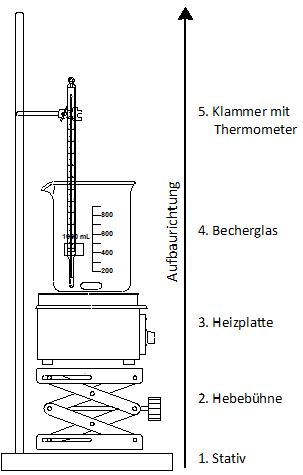
\includegraphics[width=0.4\textwidth]{img/Grundaufbau_Apparatur.png}
	\caption{Richtung für Apparaturaufbau}
\end{figure}
\FloatBarrier
%Ende

\subsubsection{Schliffklemmen alias \textsc{Keck}-Clips}
Schliffklemmen bzw. \textsc{Keck}-Clips sichern die Verbindung zwischen Glasgeräten mit Normschliff. Diese Art von Schliffsicherung findet sich vorrangig im anorganischen und organischen Chemiepraktikum für den Aufbau größerer Apparaturen. Die Ausführung der Schliffklemmen ist verschiedenen Formen und Materialien zu finden. Eine häufig vertretende Form aus Kunststoff  sind die patentierten \textsc{Keck}-Clips.

\begin{figure}[h!]
	\begin{minipage}[b]{.4\textwidth} % [b] => Ausrichtung an \caption
		\centering
		\includegraphics[width=0.6\textwidth]{img/keck_clips}
		\caption{Skizze von \textsc{Keck}-Clips}
	\end{minipage}
	\hspace{.1\linewidth}% Abstand zwischen Bilder
	\begin{minipage}[b]{.4\textwidth} % [b] => Ausrichtung an \caption
		\centering
		\includegraphics[width=0.7\textwidth]{img/keck_clips_2}
		\caption{Beispielhafte Nutzung von \textsc{Keck}-Clips}
	\end{minipage}
\end{figure}
\FloatBarrier

\textit{Tipp:}\\
\vspace*{-5mm}

\fbox{\parbox{\linewidth}{
Um kleine oder leichte Apparaturteile, wie zum Beispiel Thermometer, zu montieren ist mit solchen Klemmen keine weitere Befestigung mehr nötig.}}

\subsubsection{Muffen}
Stativmuffen sind einer der häufigsten verwendeten Bauteil im apparativen Labor. Sie werden vorzugsweise für die Befestigung von zylindrischen Stativteilen, wie einer Stativklemme oder einem Stativring.
\vspace*{-5mm}
\begin{figure}[h!]
	\centering
	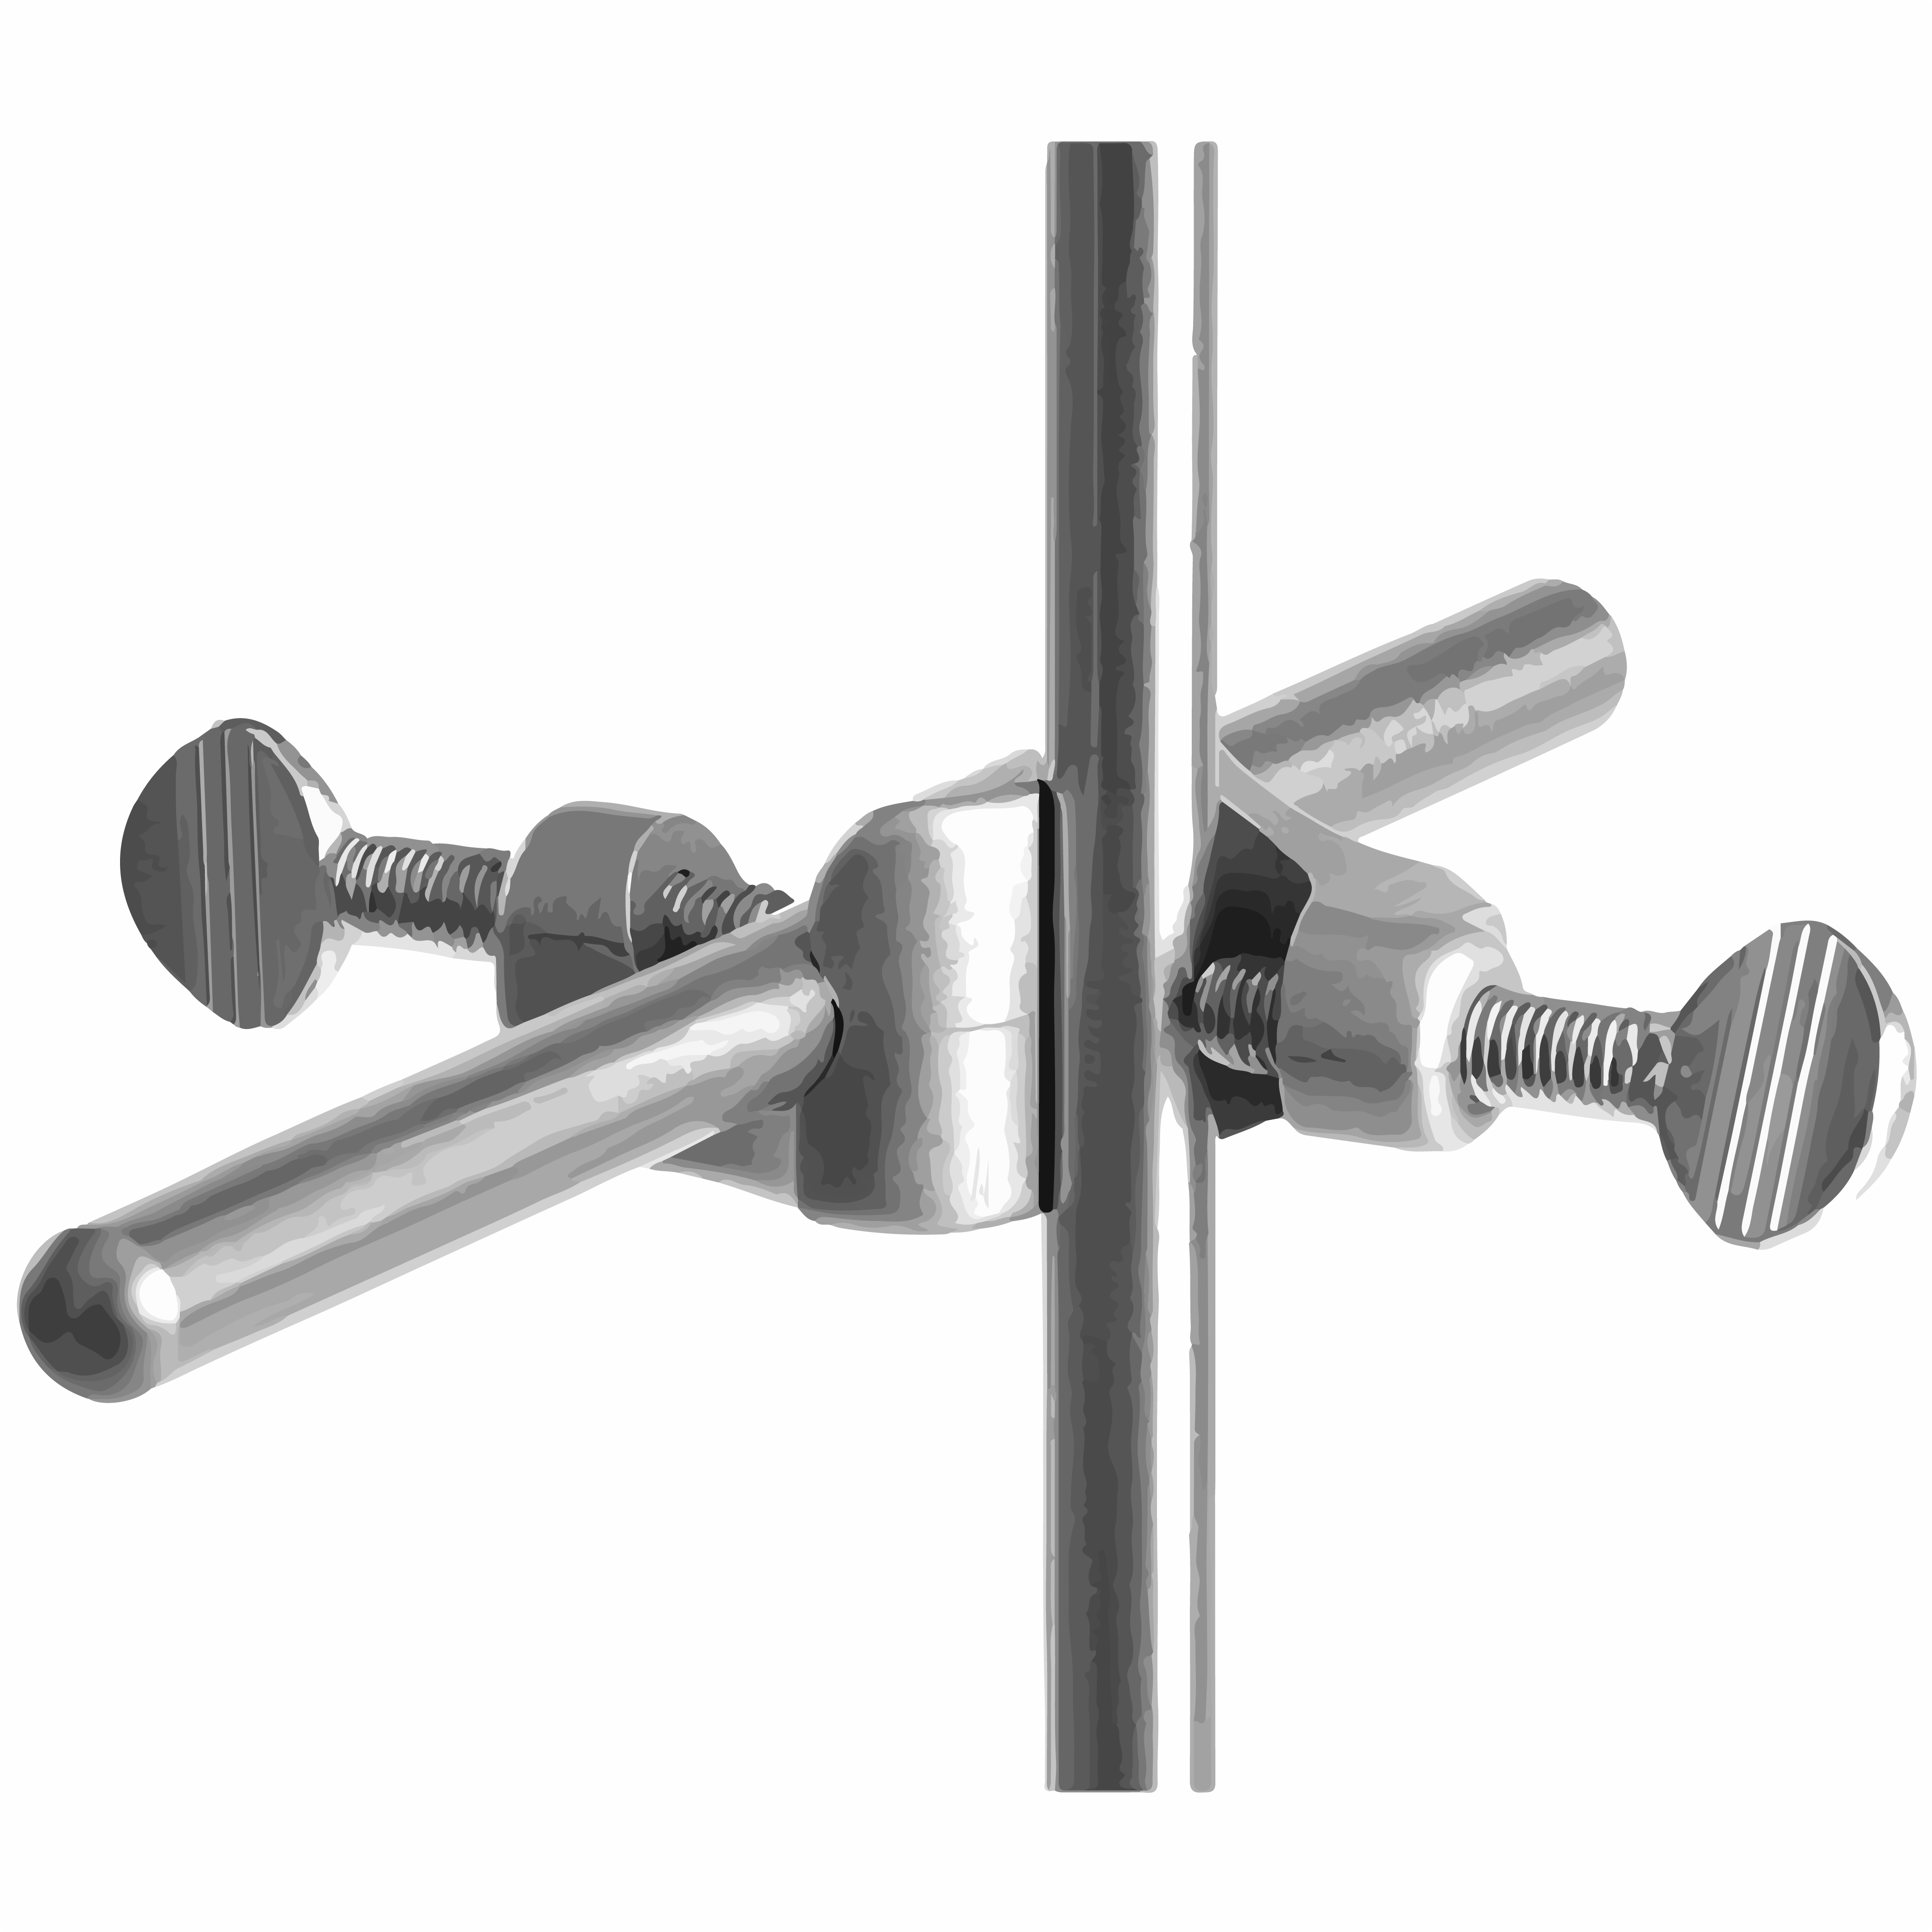
\includegraphics[width=0.3\textwidth]{img/muffe}
	\caption{Bild einer Stativmuffe}
	\label{fig:muffe}
\end{figure}
\FloatBarrier
%Ende
\vspace*{-2mm}
\subsubsection{(\textsc{Bunsen}-) Stative}
\textsc{Bunsen}-Stative bzw. Laborstative bestehen aus einer metallenen Grundplatte an welcher senkrecht eine Metallstange eingeschraubt ist. Sie dienen dazu verschiedene Versuchsaufbauten zu konstruieren indem an die die Stange mittels Muffen und Klemmen verschiedenste Hilfsmittel wie Gefäße, Büretten, Kochringe oder ähnliches in verschiedenen Höhen befestigt werden können.

\subsubsection{Korkringe}
Korkringe dienen zum Ablegen von Rundkolben, wenn diese nicht in ein Stativ eingespannt sind. Somit wird gesichert, dass Rundkolben aufgrund ihrer kugeligen Form nicht wegrollen.
\begin{figure}[h!]
	\centering
	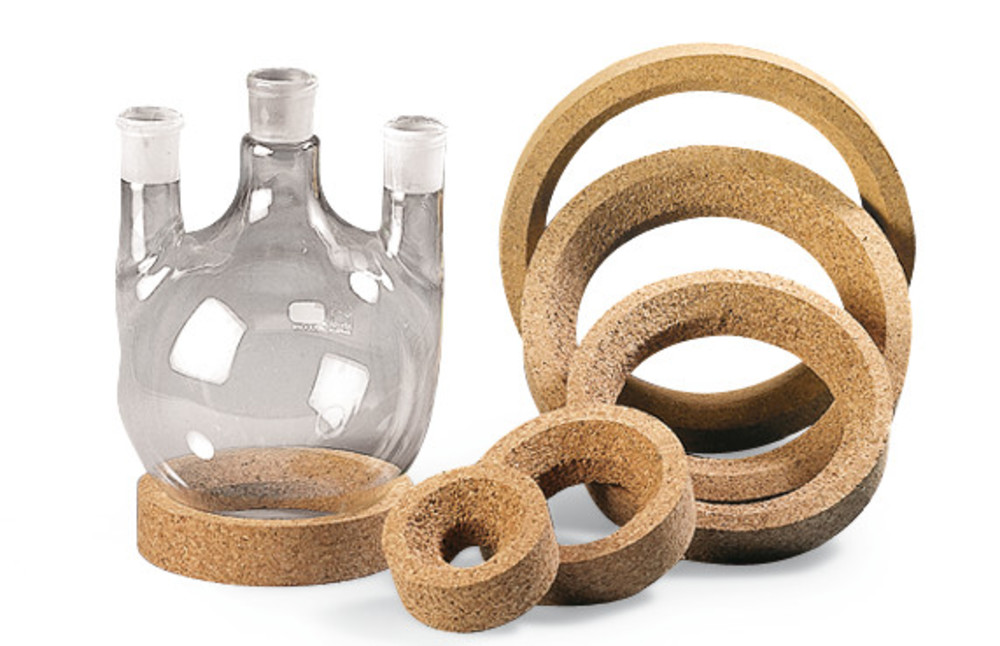
\includegraphics[width=0.45\textwidth]{img/korkring}
	\caption{Korkringe für Rundkolben}
	\label{fig:korkring}
\end{figure}
\FloatBarrier
%Ende

\subsubsection{Material der Glasgeräte}
Glasgeräte im chemischen Labor bestehen meistens aus Borosilicatglas. Es zeichnet sich durch eine hohe Temperatur- und Chemikalienbeständigkeit aus und hält somit in den Bereichen der Chemie, der Verfahrenstechnik und dem Haushalt Einzug. Typischer Markennamen für Borosilikatgläser sind beispielsweise \textsc{Jenaer Glas}, \textsc{Duran}, \textsc{Pyrex} oder \textsc{Simax}, um nur ein paar zu nennen.
Auch im großtechnischen Bereich findet das Glas seine Anwendung, wie zum Beispiel in Schauglasarmaturen, Durchflussgläsern oder Behälterschaugläsern. 
\begin{figure}[h!]
		\centering
		\begin{minipage}{0.3\textwidth}
			
\includegraphics[width=0.5\textwidth]{img/logo_duran}
		\end{minipage}
		\begin{minipage}{0.30\textwidth}
			
\includegraphics[width=0.7\textwidth]{img/logo_jenaerglas}
		\end{minipage}
		\begin{minipage}{0.30\textwidth}
			
\includegraphics[width=0.7\textwidth]{img/logo_pyrex}
		\end{minipage}
		\caption{Logos von Borosilikatglas-Herstellern}
\end{figure}
\FloatBarrier

\pagebreak

\subsection{Volumengefäße}
\subsubsection{Bechergläser}
Bechergläser sind zylindrische Becher, welche an der Oberseite einen gebogenen Rand, sowie eine Ausgussmöglichkeit haben. Sie werden für vielfältige Aufgaben, wie dem Erhitzen oder Zusammengießen von Flüssigkeiten. Es gibt sie in verschiedensten Ausführungen und Größen, welche meistens mit einem groben Maßstab versehen sind.\\
\vspace*{-5mm}

\textit{Hinweis:}\\
\vspace*{-5mm}

\fbox{\parbox{\linewidth}{
Messbecher sollten nicht genutzt werden um genaue Volumina zu messen. Besser eignen sich hierfür Messzylinder oder Maßkolben für das entsprechende Volumina.}}
\begin{figure}[h!]
	\centering
	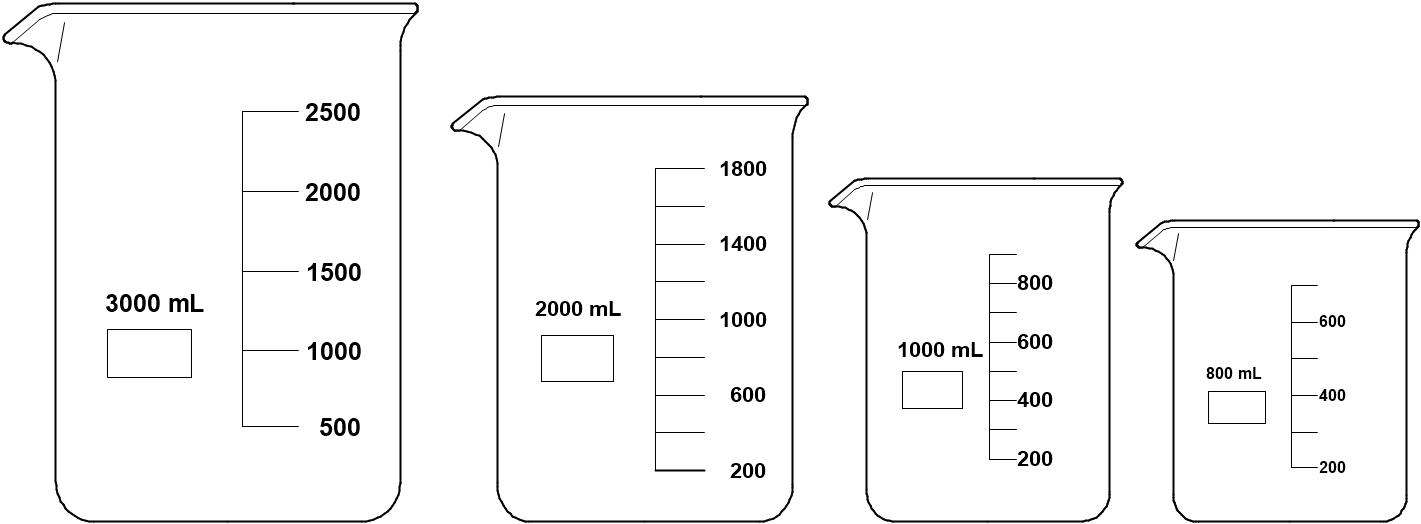
\includegraphics[width=0.45\textwidth]{img/becherglas}
	\caption{Bechergläser}
	\label{fig:becherglas}
\end{figure}
\FloatBarrier
%Ende
\vspace*{-10mm}

\subsubsection{Rundkolben}
Rundkolben werden ähnlich wie Bechergläser in den verschiedensten Größen und Ausführungen hergestellt. Viele der Kolben besitzen einen sogenannten Normschliff am Kolbenhals um beliebig und einfach gasdichte Apparaturen zusammenzustecken (mehr unter \hyperlink{Normschliff}{Normschliffe}). Des Weiteren können Rundkolben auch als Mehrhalskolben ausgeführt sein, um an den zusätzlichen Öffnungen zum Beispiel Kühler, Rührer, Messgeräte und/oder Zuläufe gleichzeitig anzubringen. Zusätzlich können Rundkolben, im Gegensatz zu Standkolben auch unter Vakuum genutzt werden, da die runde Form eine Implosion verhindert. Diese runde Form ermöglicht ebenfalls ein gleichmäßiges Erwärmen des Kolbeninhaltes.
\begin{figure}[h!]
	\centering
	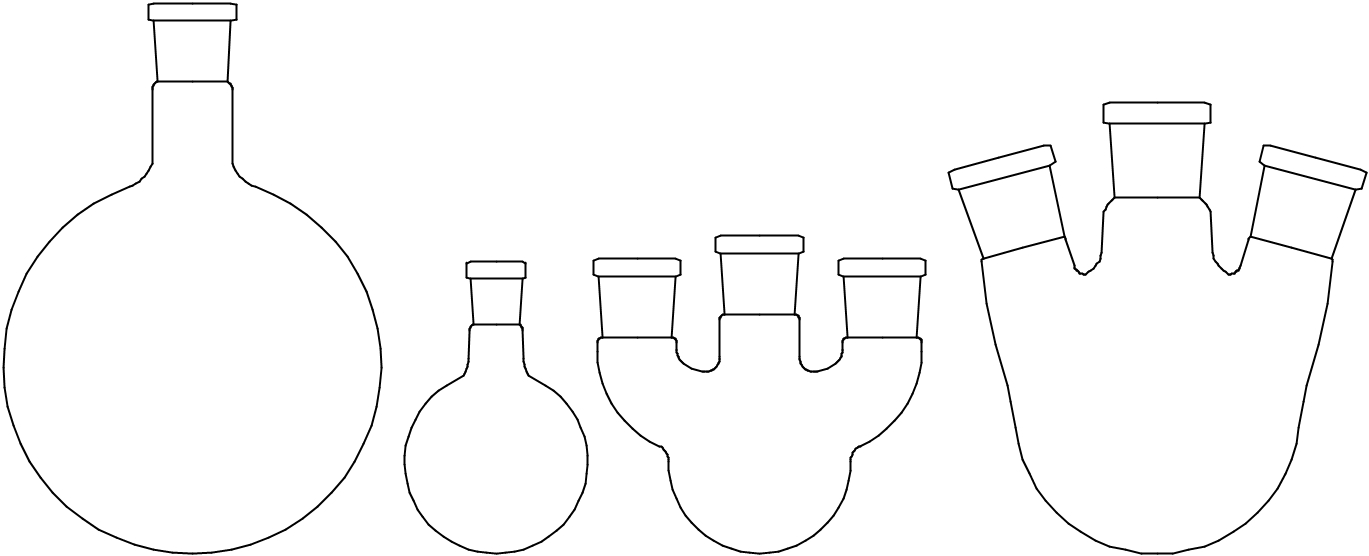
\includegraphics[width=0.45\textwidth]{img/rundkolben}
	\caption{Rund- und Mehrhalskolben}
	\label{fig:rundkolben}
\end{figure}
\FloatBarrier
%Ende

\subsubsection{Standkolben: Erlenmeyerkolben und Stehkolben}
Erlenmeyerkolben und Stehkolben unterscheiden sich im zum Becherglas vor allem im nach oben hin enger werdenden Hals. Dieser kann ebenfalls, wie bei den Rundkolben, je nach Anwendung mit einem Normschliff versehen sein. Gerade Erlenmeyerkolben werden aufgrund der Unterschiedlichen Ausführung des Kolbenhalses weiter in Enghals- und Weithalskolben klassifiziert. Der verjüngende Hals dieser Kolben minimiert maßgeblich die Gefahr, dass bei Zugabe von Substanzen, beim Schwenken, Rühren oder Sieden Flüssigkeiten unkontrolliert aus dem Kolben entweichen. 
Der Erlenmeyerkolben besticht dabei durch die Möglichkeit, die enthaltene Flüssigkeit gut zu Schwenken zu können, während der Stehkolben einen Rundkolben darstellt, welcher nicht wegrollen kann und eine druckstabiliere Bauweise glänzt.

\begin{figure}[h!]
	\centering
	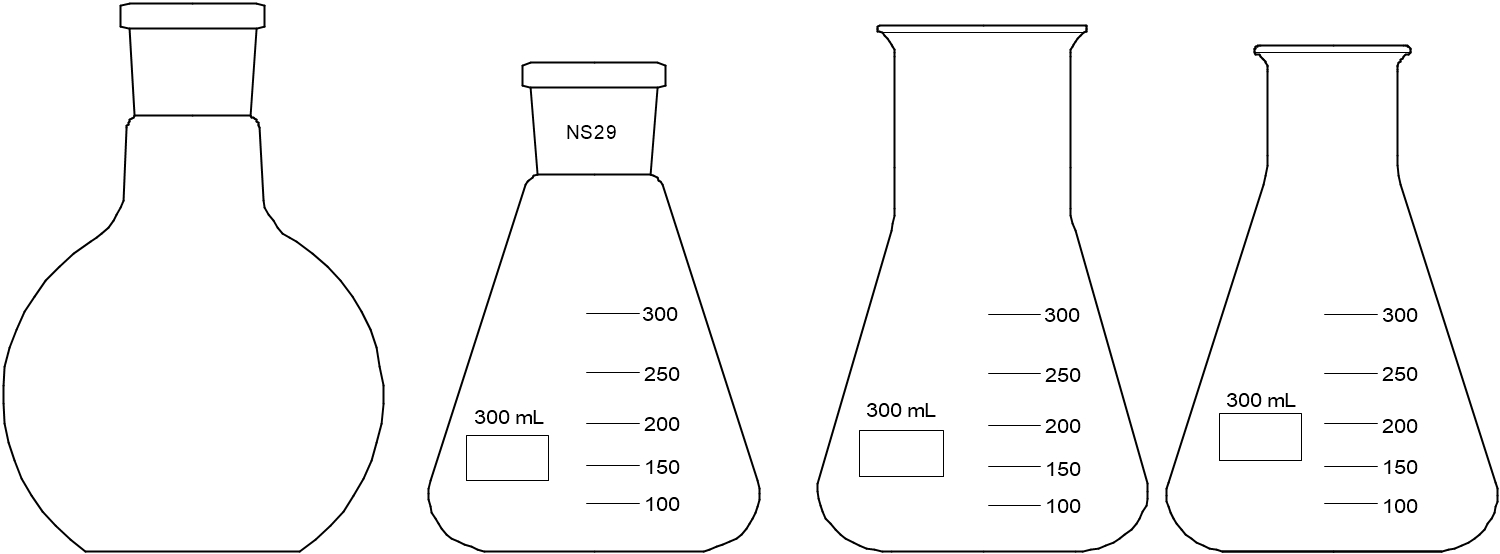
\includegraphics[width=0.65\textwidth]{img/standkolben}
	\caption{Standkolben}
	\label{fig:standkolben}
\end{figure}
\FloatBarrier
%Ende

\begin{table}[h!]
	\renewcommand*{\arraystretch}{1.2}
	\centering
	%\rowcolors{2}{white}{gray!25}
	\caption{Vergleich von Becherglas, Rund- und Standkolben}
	\label{tab:vergleich_becherglas}
	\resizebox{15cm}{!}{
		\begin{tabulary}{1.2\textwidth}{C|C|C|C|C}
			\hline
			 \diagbox{Eigenschaft:}{Kolben:}& \textbf{Becherglas} & \textbf{Rundkolben} &\textbf{Rundkolben}& \textbf{Erlenmeyer}\\
			\hline
			Magnetrührer & ja &ja & ja&ja\\
			hitzebeständig & ja &ja & ja&ja\\
			Mischung von Flüssigkeiten & ja &ja & ja&ja\\
			\hline
			selbststehend &ja&nein&ja&ja\\
			Normschliff &nein&ja&ja&ja\\
			gleichmäßiges Erwärmen &nein&ja&nein&nein\\
			vakuumfest &nein&ja&nein&nein\\
			\hline      
	\end{tabulary}}
\end{table}%
\FloatBarrier

\newpage

\subsubsection{Maßkolben bzw. Messkolben}
Maßkolben dienen hauptsächlich zum Ansetzen und Aufbewahren von Maßlösungen mit exakten Konzentrationen. Sie sind auf Einguss geeicht und zählen somit nicht unter die Kategorie Volumenmessgerät!\\
{\small Unter Maßlösungen versteht man Lösungen mit einer genau bestimmten Menge einer Substanz, welche über einen Urtiter oder Vergleichslösungen bestimmt wird. Urtiter wiederum die gut wägbare Reinsubtanzen mit welchen sich der Gehalt von Maßlösungen bestimmen lässt.}

\begin{figure}[h!]
	\centering
	\includegraphics[width=0.12\textwidth]{img/Messkolben}
	\caption{Maß- bzw. Messkolben}
	\label{fig:messkolben}
\end{figure}
\FloatBarrier


\subsection{Messzylinder}
Ein Messzylinder ist ein senkrechter, hoher Glas- oder Plastikzylinder mit einem Standfuß. Über eine aufgebrachte Skala können ihm Volumina abgemessen werden. Er ist genauer als ein Becherglas, aber ungenauer als eine Voll- oder Kolbenhubpipette (\textsc{Eppendorf}-Pipette). Je nach dem wie wichtig das genaue Abmaß des Volumens sein muss, sollte auf die aufgedruckte Fehlerklasse bzw. Fehlertoleranz geachtet werden.

\begin{figure}[h!]
	\centering
	\includegraphics[width=0.27\textwidth]{img/Messzylinder}
	\caption{Messzylinder}
	\label{fig:messzylinder}
\end{figure}
\FloatBarrier

\newpage


\subsubsection{Bürette}
Eine Bürette ist eine kalibrierte, skalierte Glasröhre mit einem Hahn am unteren Ende und dient zur quantitativen Abmessung von geringen Flüssigkeitsvolumina für Titrationen. Eine besondere Form der Bürette ist die automatische Bürette bei der über einen Blasebalg aus einem Vorratsbehälter der Messzylinderteil der Bürette wieder aufgefüllt wird (siehe Abb. \ref{fig:bürette}).

\begin{figure}[h!]
	\centering
	\includegraphics[width=0.5\textwidth]{img/bürette_beide}
	\caption{normale und automatische Bürette}
	\label{fig:bürette}
\end{figure}
\FloatBarrier

\textit{Wichtig:}\\
\vspace*{-5mm}

\fbox{\parbox{\linewidth}{
		Das Luftloch der automatischen Bürette sollte nicht zugehalten werden, da sich sonst ein zerstörerischer Druck im Vorratsbehälter aufbauen kann!}}
	
	\vspace*{5mm}
	
	\textit{Hinweis:}\\
	\vspace*{-5mm}
	
	\fbox{\parbox{\linewidth}{Vor Einsatz der Bürette sollte geprüft werden ob der Hahn nur schwergängig nutzbar ist. Ist dies der Fall sollte der Hahn mit mit Schlifffett gefettet werden.}}
	
	\newpage

\subsection{Pipetten}
\subsubsection*{Peleusball}
\begin{figure}[h!]
	\begin{minipage}[t]{0.73\textwidth}
		\vspace{0pt}
		Der Peleusball ist eine gummierte Pipettierhilfe mit welcher das Abmessen von Flüssigkeitsvolumina in Glaspipetten ermöglicht wird. Hierfür wird der Auslass A geöffnet (zusammendrücken) und der Ball selbst zusammengedrückt, um einen Unterdruck zu erzeugen. Drückt man nun auf das Saugventil S wird die Flüssigkeit in die Glaspipette gesaugt und über drücken des Ventils E kann diese Flüssigkeit kontrolliert abgegeben werden.
	\end{minipage}
	\hfill
	%\hspace{1mm}
	\begin{minipage}[t]{0.25\textwidth}
		\vspace{0pt}
		\centering
		\includegraphics[angle=90,width=0.4\textwidth]{img/peleusball}
		\caption{Peleusball}
		\label{fig:peleus}
	\end{minipage}
\end{figure}
\FloatBarrier

\subsubsection*{Vollpipetten}

\begin{figure}[h!]
	\begin{minipage}[t]{0.25\textwidth}
		\vspace{0pt}
		\centering
		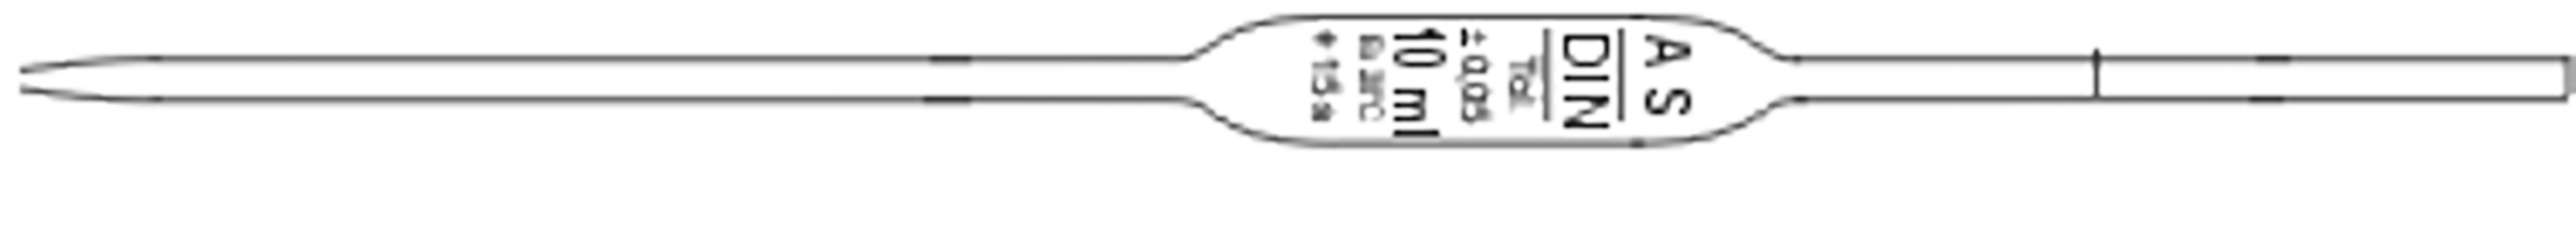
\includegraphics[angle=90,width=0.088\textwidth]{img/vollpipette}
		\caption{Vollpipette}
		\label{fig:vollpipette}
	\end{minipage}
	\hfill
	\hspace{1mm}
	\begin{minipage}[t]{0.75\textwidth}
		\vspace{0pt}
		Vollpipetten sind kalibrierte Glasröhrchen mit einer Glasblase, um genaue Dosierungen Flüssigkeitsvolumina abzumessen.  Sie sind auf Ausguss geeicht und besitzen ebenfalls, wie die Messzylinder eine aufgedruckte Fehlertoleranz oder Fehlerklasse. Typische Volumina für Vollpipetten sind \SI{5}{\milli \liter}, \SI{10}{\milli \liter}, \SI{20}{\milli \liter }, \SI{50}{\milli \liter } und \SI{100}{\milli \liter}. Daher sind Vollpipetten hervorragend für für Volumenabmessungen in den genannten Bereichen geeignet. Für geringere Volumina im Mikroliterbereich sollten Hubkolbenpipetten genutzt werden.
	\end{minipage}
\end{figure}
\FloatBarrier

\subsubsection*{Kolbenhubpipette bzw. Eppendorfpipetten}
\begin{figure}[h!]
	\begin{minipage}[t]{0.63\textwidth}
		\vspace{0pt}
		Kolbenhubpipetten, auch Mikroliter- oder Mikropipette genannt, sind mechanische Pipetten, welche Volumina in Dosierungen von \SI{0,1}{\micro \liter} bis \SI{5}{\milli \liter}  genauer als herkömmliche Glaspipetten dosieren können. Durch den bewegten Kolben beim Herunterdrücken wird in der aufgesteckten Pipettenspitze ein Unterdruck erzeugt, welcher die Flüssigkeit in die Spitze zieht. Die Menge an Volumen, die durch die Pipette angesaugt wird, ist meist über einen Drehmechanismus an der Pipette einstellbar.\\
		Eine verbreitete Bezeichnung für diese Pipetten ist \mbox{\textsc{Eppendorf}}-Pipette, wobei \textsc{Eppendorf} die Marke des Pipettenherstellers beschreibt und nicht die Ausführung der Pipette.
	\end{minipage}
	\hfill
	%\hspace{1mm}
	\begin{minipage}[t]{0.35\textwidth}
		\vspace{0pt}
		\centering
		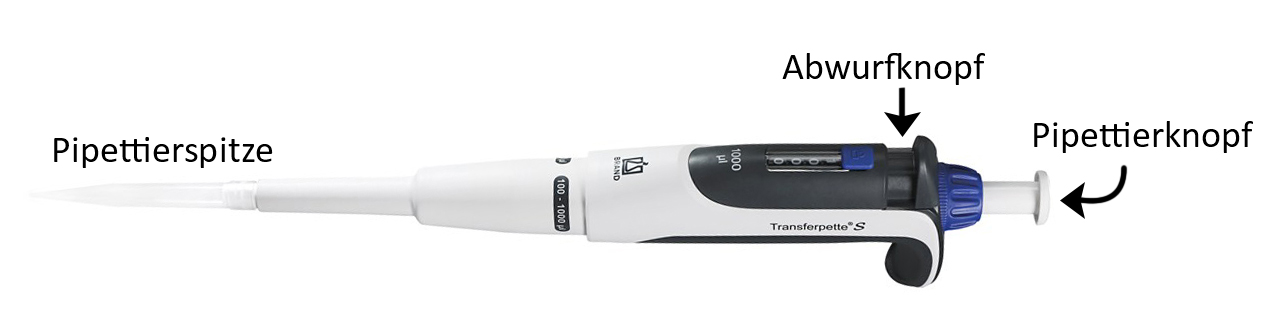
\includegraphics[angle=90, width=0.33\textwidth]{img/eppendorf}
		\caption{Kolbenhubpipette}
		\label{fig:eppen}
	\end{minipage}
\end{figure}
\FloatBarrier

\textit{Benutzung:}\\
\vspace*{-5mm}

%Volumen auf und abgabe oberseitenknopf
%Hinweis wegen pipetten spitze abwurf großer Knop

\fbox{\parbox{\linewidth}{
\textbf{Volumenaufnahme:}
\begin{enumerate}
	\item Pipettierknopf bis zum ersten Anschlagdrücken
	\item Pipettenspitze in die Flüssigkeit tauchen
	\item Pipettierknopf langsam hochziehen (ohne Luft!)\\
	$\rightarrow$ es dürfen keine Luftblasen in der Pipettenspitze sein 
\end{enumerate}
\textbf{Volumenabgabe:}
\begin{enumerate}
	\item Pipettenspitze an die Innenwand des Gefäßes halten
	\item Pipettierknopf langsam bis zum zweiten Anschlag drücken
\end{enumerate}

Die Pipettenspitze kann über den großen, forderen Abwurfknopf entfernt werden.
}}

\begin{figure}[h!]
	\centering
	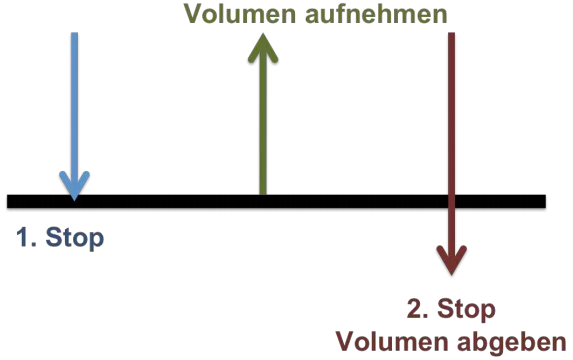
\includegraphics[width=0.45\textwidth]{img/volumen_eppendorf}
	\caption{Schematische Umgangsweise mit einer Kolbenhubpipette}
	\label{fig:eppen_Vol}
\end{figure}
\FloatBarrier

\subsection{Trichter}
\subsubsection*{Flüssigkeitstrichter}
\begin{figure}[h!]
	\begin{minipage}[t]{0.63\textwidth}
		\vspace{0pt}
		Flüssigkeitstrichter sind Geräte, ein mit großer Öffnung und kleiner Mündung mit welchem sich Flüssigkeiten in Gefäße mit kleiner Mündung, wie Flaschen, Erlenmeyer- und Rundkolben gießen lassen. Sie bestehen meist aus Glas, Kunststoff und in selteneren Fällen auch aus Metall.
	\end{minipage}
	\hfill
	%\hspace{1mm}
	\begin{minipage}[t]{0.35\textwidth}
		\vspace{0pt}
		\centering
		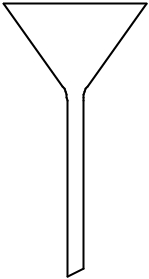
\includegraphics[width=0.25\textwidth]{img/trichter}
		\caption{Flüssigkeitstrichter}
		\label{fig:flussigtrichter}
	\end{minipage}
\end{figure}
\FloatBarrier

\subsubsection*{Feststoff- bzw. Pulvertrichter}
Pulvertrichter werden, wie der Name vermuten lässt, für das Abfüllen von Pulvern, Granulaten oder feinkristallinen Stoffen genutzt. Sie unterscheiden sich gegenüber den Flüssigkeitstrichter in der Tatsache, dass das Verhältnis zwischen dem Durchmesser der Öffnung und der Mündung des Trichter größer ausfällt.
Gerade für zittrige Hände kann ein Feststofftrichter helfen das Schüttgut in den entsprechenden Behälter ohne größere Verluste zu überführen.
\begin{figure}[h!]
	\centering
	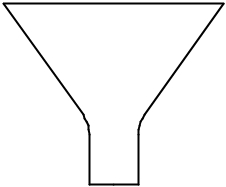
\includegraphics[ width=0.2\textwidth]{img/trichter2}
	\caption{Pulvertrichter}
	\label{fig:pulvertrichter}
\end{figure}
\FloatBarrier

\subsubsection*{Tropftrichter} 
 \begin{figure}[h!]
 	\begin{minipage}[t]{0.30\textwidth}
 		\vspace{0pt}
 		\centering
 		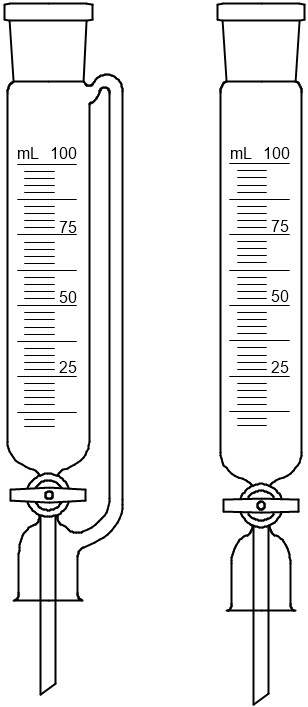
\includegraphics[width=0.6\textwidth]{img/tropftrichter}
 		\caption{Tropftrichter mit und ohne Druckausgleich}
 		\label{fig:tropftrichter}
 	\end{minipage}
 	\hfill
 	\hspace{1mm}
 	\begin{minipage}[t]{0.7\textwidth}
 		\vspace{0pt}
 		Tropftrichter sind Glasgeräte, welche hauptsächlich im chemischen Labor für die tropfenweise Zugdosierung von Chemikalien in eine Reaktionsmischung dienen. Sie besitzen meist einen Normschliff und es gibt sie in Ausführungen mit und ohne Druckausgleich. Mit Druckausgleich am Tropftrichter wird ein Verdampfen der zuzutropfenden Lösung vermieden. Auch hier ist darauf zu achten, dass zum Dosieren der Hahn des Tropftrichters zuvor mit Schlifffett zu behandeln ist. Die angebrachte Skalierung am Tropftrichter ist als Richtwert zu verstehen. Genaue Volumina sollten mittels Messzylinder oder Pipetten abgemessen werden.
 	\end{minipage}
 \end{figure}
 \FloatBarrier
 
 \newpage
 
\subsubsection*{Scheidetrichter bzw. Schütteltrichter}
\begin{figure}[h!]
	\begin{minipage}[t]{0.68\textwidth}
		\vspace{0pt}
		Scheidetrichter sind Glasbehälter, welche zur Trennung von nicht mischbaren Flüssigkeiten dienen. Bei verschlossenem Hahn wird über den Normschliff an der Oberseite das zu trennende Flüssigkeitsgemisch eingefüllt. Der Normschliff wird mit einem Stopfen verschlossen und die Phase mit größeren Dichten sammelt sich am Ende des Scheidetrichters. Diese Phase kann nun über den Hahn des Trichters abgegossen werden. Die konische Form des Scheidetrichters erleichtert dabei die Arbeit einer exakten Abtrennung.\\
		Scheidetrichter werden deshalb gerne auch für Flüssig-Flüssig-Extraktionen genutzt, aus welchen sich der Begriff des "`Ausschüttelns"' ergibt \mbox{(siehe \ref{sec:extraktion})}.
	\end{minipage}
	\hfill
	%\hspace{1mm}
	\begin{minipage}[t]{0.30\textwidth}
		\vspace{0pt}
		\centering
		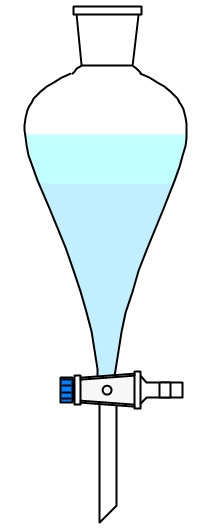
\includegraphics[width=0.51\textwidth]{img/scheidetrichter}
		\caption{Scheidetrichter}
		\label{fig:scheidetrichter}
	\end{minipage}
\end{figure}
\FloatBarrier
\vspace{-7mm}
\subsection{Schläuche}
\subsubsection*{Wasserschläuche}
\begin{figure}[h!]
	\begin{minipage}[t]{0.63\textwidth}
		\vspace{0pt}
		Wasserschläuche im chemischen Labor bestehen meist aus Silikon, Polyethylen (PE) oder Polyvinylchlorid (PVC). Sie zeichnen sich dadurch aus, dass sie durchsichtig sind, hitzebeständig bis mindestens \SI{100}{\celsius} sowie universal, chemisch beständig sind. 
		Sie besitzen meist Wandstärken von 1-\SI{2}{\milli \meter} und werden im chemischen Labor vorzugsweise für den Anschluss von Thermostaten, sowie jegliche Art von Wasserkühlern genutzt.
	\end{minipage}
	\hfill
	\hspace{1mm}
	\begin{minipage}[t]{0.35\textwidth}
		\minibild{Wasserschlauch}{1}{0pt}
	\end{minipage}
\end{figure}
\FloatBarrier
\vspace{-7mm}
\subsubsection*{Vakuumschläuche}
 \begin{figure}[h!]
	\begin{minipage}[t]{0.35\textwidth}
		\minibild{Vakuumschlauch}{1}{0pt}
	\end{minipage}
	\hfill
	\hspace{2mm}
	\begin{minipage}[t]{0.65\textwidth}
		\vspace{0pt}
		Vakuumschläuche werden im chemischen Labor für jegliche Anwendungen genutzt in denen ein Vakuum gezogen wird. Das betrifft in den meisten Fällen die Vakuumfiltration mittels Saugflasche und Filternutsche bzw. Fritte. Sie bestehen häufig aus Naturkautschuk (NR: natural rubber) und besitzen in der Regel eine Wandstärke von \SI{4}{\milli \meter}. Naturkautschuk findet in diesen Schläuchen Anwendung, da dieser gegenüber synthetisch hergestellten Kautschuk höhere Verschleißfestigkeit, Alters und Witterungsbeständigkeit besitzt, jedoch wird dieser im Gegensatz zu Kunststoffen wie Silikon mit der Zeit brüchig.
	\end{minipage}
\end{figure}
\FloatBarrier

\tipp{Tipp}{Wenn Schläuche an den Enden sehr abgenutzt oder brüchig aussehen, müssen diese nicht entsorgt, sondern lediglich das Ende mit einer (Universal)-Schere abgeschnitten werden.}
\vspace{5mm}

\subsubsection{Oliven}
Schlaucholiven sind Übergangsstücke für Schläuche. Sie können aus Glas, Metall oder Kunststoff sein und sind meist als Anschlussstück für den Schlauch an eine Apparatur wiederzufinden oder als Übergangsstück um zwei Schläuche gleichen oder unterschiedlichen Durchmessers miteinander zu verbinden.

\bild{Olive}{0.5}

\subsection{Filter}
\subsubsection*{Filterpapier}
Filterpapier besteht meist aus verschiedenen Faserschichten wie Baumwolle, Cellulose oder Glas. Diese Schichten halten je nach Güteklasse die Feststoffteilchen bis zu einem bestimmten Partikeldurchmesser an der Oberfläche und im Innern des Filters zurück. Als Filterpapiere kommen im Regelfall Papierfilter (Rund- oder Faltenfilter) zum Einsatz. Diese sind für die Filtration von verdünnten Säuren, Laugen oder anderen Lösungsmitteln in den meisten Fällen ausreichend. Es gibt jedoch auch weitere Filterpapiere wie Normalpapiere, Hartfilter oder aschefreie Filter, welche speziellere Anwendungen ausgelegt sind.\\
\newpage

\textit{Güteklassen für qualitatives Filterpapier aus Cellulose (Rundfilter):}

	\begin{itemize}
		\item \textbf{GK1 $\left[\SI{11}{\micro \meter}\right]$:} \\
		Mittleres Partikelrückhaltevermögen (Retention) und Fließgeschwindigkeit für Routinelaborarbeiten		
		\item \textbf{GK2 $\left[\SI{8}{\micro \meter}\right]$:}\\
		Mehr Rückhaltevermögen als GK1, aber mit geringerer Fließgeschwindigkeit
		\item \textbf{GK3 $\left[\SI{6}{\micro \meter}\right]$:}\\
		Dickes Papier mit hoher Belastbarkeit, welches sich besonders für den \textsc{Büchner}-Trichter eignet
		\item \textbf{GK4 $\left[\text{20}-\SI{25}{\micro \meter}\right]$:}\\
		Hohe Durchflussgeschwindigkeit für größere Partikel und gelartige Niederschläge
		\item \textbf{GK5 $\left[\SI{2,5}{\micro \meter}\right]$:}\\ wirkungsvollstes, quantitatives Papier für kleinste Partikel
		\item \textbf{GK6 $\left[\SI{3}{\micro \meter}\right]$:} doppelt so schnell wie GK5, aber geringfügig schlechterer Partikelrückhalt
\end{itemize}

%https://www.myneolab.de/83/1/VP45/250206806/250206806+VGKL%20Seite.html
%https://www.cytivalifesciences.com/en/us/solutions/lab-filtration/knowledge-center/a-guide-to-whatman-filter-paper-grades

\subsubsection*{Fritte}
Eine Fritte ist ein Filter aus Glas oder Keramik, welcher zum Filtern von feinen Partikeln genutzt wird. Das entsprechende Glas bzw. die Keramik ist dabei so porös, dass sie ähnlich einem sehr feinen Sieb wirken. Typische Fritten lassen sich mit ISO P500, P100, P40 und P1,6 bezeichnen.

\subsubsection*{Filternutsche alias \textsc{Büchner}-Trichter}
\begin{figure}[h!]
	\begin{minipage}[t]{0.7\textwidth}
		\vspace{0pt}
		Die Filternutsche, auch \textsc{Büchner}-Trichter genannt, ist ein mechanischer Filter zur Trennung von Suspensionen. Sie wird zusammen mit einer Saugflasche zur Saugfiltration genutzt. Hierbei ist es nötig ein entsprechendes Filterpapier zurecht zuschneiden und in den Trichter einzulegen. Nach der Filtration kann dann das Filterpapier zusammen mit dem Filterkuchen wieder entnommen werden.
	\end{minipage}
	\hfill
	\hspace{1mm}
	\begin{minipage}[t]{0.25\textwidth}
		\minibild{Nutsche}{0.85}{0pt}
	\end{minipage}
\end{figure}
\FloatBarrier

\tipp{Tipp}{Um zu Prüfen ob an der aufgebauten Saugfiltration der benötigte Unterdruck anliegt, kann ein Stück bedeckendes Papier über den Trichter gelegt werden. Liegt ein ausreichender Unterdruck an verformt sich das Papier.}\\

\subsubsection*{Watte oder Glaswolle}
\begin{figure}[h!]
	\begin{minipage}[t]{0.3\textwidth}
		\minibild{Watte}{0.44}{0pt}
	\end{minipage}
	\hfill
	\hspace{2mm}
	\begin{minipage}[t]{0.7\textwidth}
		\vspace{0pt}
		Sollen lediglich geringe Mengen an Feststoff oder Niederschlägen von einer Lösung grob getrennt werden, so ist es möglich statt Filterpapier auch Watte in einem Trichter zu nutzen. Gerade im organisch-chemischen Labor kommt es dazu, dass geringe Feststoffabfälle vom zu entsorgenden Lösemittel getrennt werden, um die allgemeine Entsorgung zu vereinfachen. Glaswolle ist handelsüblicher Watte dann vorzuziehen, sobald zusätzliche thermische oder chemische Beständigkeit gefragt ist.
	\end{minipage}
\end{figure}
\FloatBarrier

\subsection{Waschflaschen}
Waschflaschen sind Laborgeräte, welche zum Einsatz kommen sobald ein Gasstrom in die Apparatur hinein oder aus die Apparatur heraus benötigt wird. Sie werden zwischen zwischen Pumpe und der eigentlichen Apparatur geschaltet. \\
Wie der Name schon vermuten lässt werden in in diesen Flaschen Gase gewaschen. Dies erfolgt in der Regel mit einem Lösungsmittel innerhalb der Waschflasche durch die das Gas mittels Tauchrohr geführt wird.\\
Aber auch bei der Vakuumfiltration werden Waschflaschen eingesetzt. Hierbei wird die jeweilige Waschflasche so zwischen Pumpe und Filtration geschaltet, dass äußersten Fall kein Filtrat in die Pumpe gelangt, sondern vorerst in der Waschflasche aufgefangen wird.

\begin{figure}[h!]
	\begin{minipage}[t]{0.49\textwidth}
		\vspace{0pt}
		\centering
		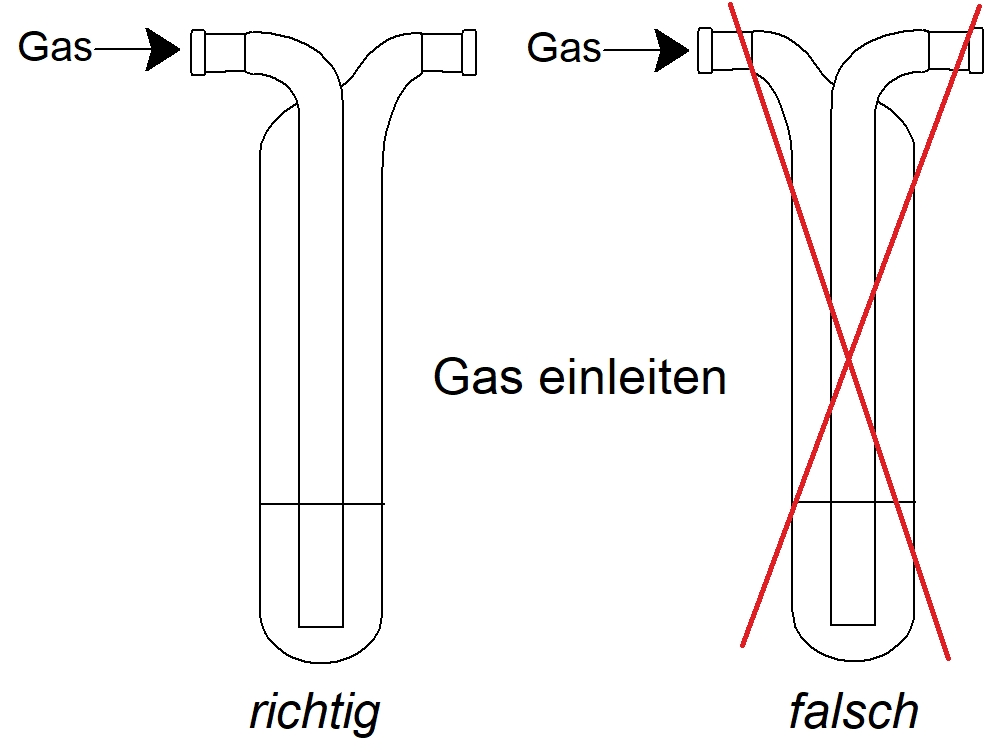
\includegraphics[width=0.9\textwidth]{img/Waschflasche (Gas einleiten).jpg}
		\caption{Waschflasche (Gas einleiten)}
		\label{fig:Waschflasche_ein}
	\end{minipage}
	\hfill
	\hspace{2mm}
	\begin{minipage}[t]{0.49\textwidth}
		\vspace{0pt}
	\centering
	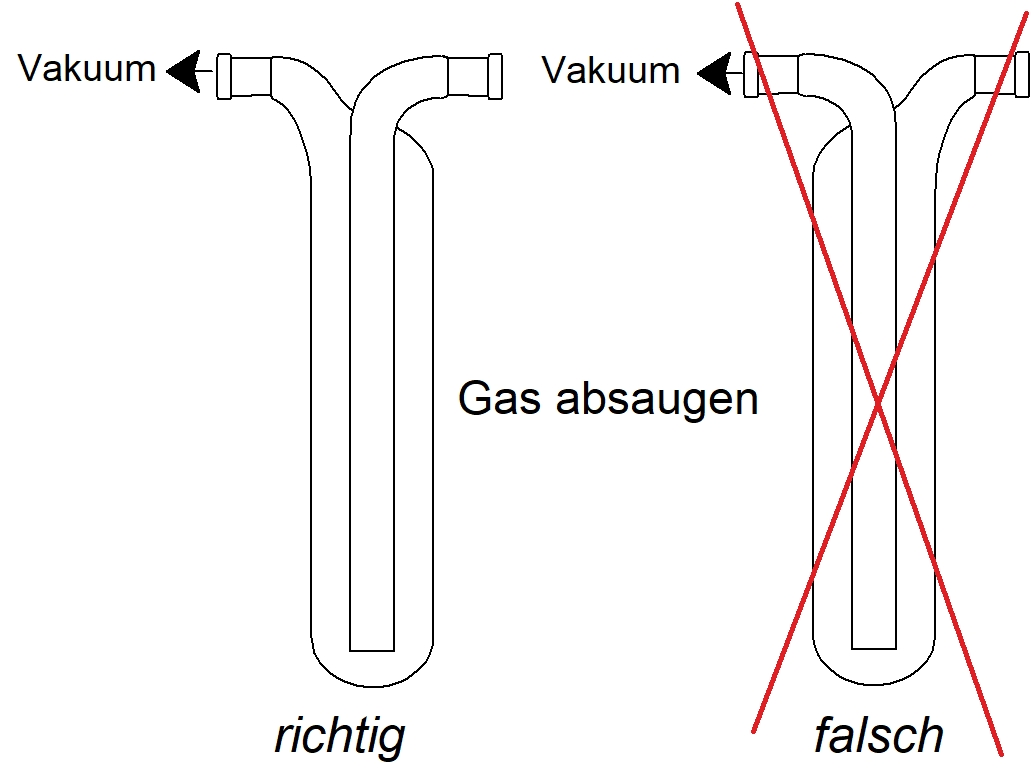
\includegraphics[width=0.9\textwidth]{img/Waschflasche (Gas absaugen).jpg}
	\caption{Waschflasche (Gas absaugen)}
	\label{fig:Waschflasche_aus}
	\end{minipage}
\end{figure}
\FloatBarrier

\subsection{Rührer}
\subsubsection*{Magnetrührwerk}
\begin{figure}[h!]
	\begin{minipage}[t]{0.6\textwidth}
		\vspace{0pt}
		Magnetrührer sind elektrische Geräte, welche oft in Kombination mit Heizplatten versehen sind. Sie werden im chemischen Labor zum Rühren von wässrigen Lösungen und Suspensionen verwendet indem ein sich ein sogenannter \textit{Rührfisch} als Dauermagnet in einem sich rotierenden Magnetfeld dreht. Die Rührgeschwindigkeit lässt sich über die Rotationsgeschwindigkeit des Magnetfeldes regeln.
	\end{minipage}
	\hfill
	\hspace{1mm}
	\begin{minipage}[t]{0.35\textwidth}
		\vspace{0pt}
		\centering
		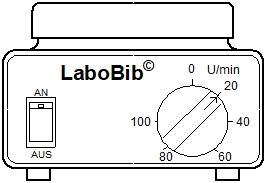
\includegraphics[width=0.88\textwidth]{img/magnetruehrer}
		\caption{Magnetrührwerk}
		\label{fig:magnetruehrwerk}
	\end{minipage}
\end{figure}
\FloatBarrier
	Der \textit{Rührfisch} ist meist mit Kunststoff oder Glas umschlossen, um ihn chemisch inert zu machen und die Reibung zu vermindern. Zusätzlich gibt es sie je nach Anwendung in verschiedenen Größen und Formen. 

\newpage

\subsubsection*{Laborrührer}
\begin{figure}[h!]
	\begin{minipage}[t]{0.65\textwidth}
		\vspace{0pt}
		Laborrührer sind ebenfalls elektrische Geräte im Labor, welche jedoch vermehrt im verfahrenstechnischen Labor als im chemischen Labor genutzt werden. Sie erfüllen dort im Labormaßstab die Grundoperationen des Lösens, Homogenisierens, Suspendierens oder Begasens. Aber auch für hochviskose Stoffe im chemischen Labor eignet sich ein solcher Rührer.\\
		Der Rührantrieb selbst ist mit einer Einspannvorrichtung, ähnlich einer Bohrmaschine, versehen. In dieser kann eine Rührwelle mit Rührblatt eingesetzt werden.
	\end{minipage}
	\hfill
	\hspace{1mm}
	\begin{minipage}[t]{0.3\textwidth}
		\vspace{0pt}
		\centering
		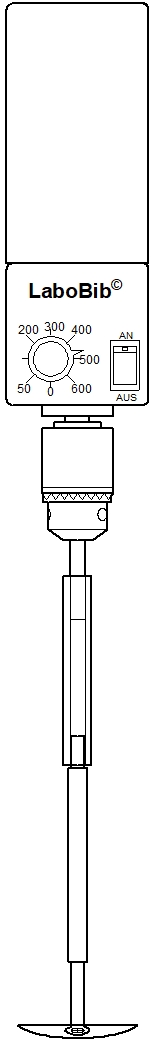
\includegraphics[height=5cm]{img/laborruehrer}
		\caption{Laborrührer}
		\label{fig:laborruehrer}
	\end{minipage}
\end{figure}
\FloatBarrier

\subsubsection*{Rührertypen}
Je nach Anwendung gibt es verschiedene Rührertypen um unterschiedliche zu erfüllen. \\
Im chemischen Labor kommen am häufigsten als zylindrische oder ovale Dauermagneten in Form von Rührfischen vor. Dabei werden zylindrische Rührfische hauptsächlich für flache Gefäße, wie Bechergläser oder Erlenmeyerkolben genutzt, während ovale Rührfische vorwiegend für Rundkolben genutzt werden. Es dennoch weitere Rührfischtypen, welche für spezielle Anwendungen ausgelegt sind, wie beispielsweise ein Kreuzrührfisch.\\
Im Verfahrenstechnischen Labor finden sich im Vergleich noch einmal deutlich mehr Rührertypen, da diese auch verfahrenstechnische Aufgaben, wie das Suspendieren oder Homogenisieren zu erfüllen haben.
Diese werden im Gegensatz zu Rührfischen mit Laborrührer, statt mit Magnetrührern in Rotation versetzt. Typische Rührertypen mit ihrer Förderrichtung und deren Anwendungszwecke finden sich in der folgenden Übersicht:
\begin{table}[h!]
	\renewcommand*{\arraystretch}{1.2}
	\centering
	%\rowcolors{2}{white}{gray!25}
	\caption{Übersicht Rührertypen}
	\label{tab:ruehrertypen}
	\resizebox{\textwidth}{!}{
		\begin{tabulary}{1.4\textwidth}{L|CCCCC}
			\hline
			\textbf{Rührertypen} & \textbf{Propeller} & \textbf{Scheibenrührer}&\textbf{Schrägblattrührer} & \textbf{Ankerrührer}&\textbf{Wendelrührer}\\
			\hline
			\textbf{Bilder} &&&&&\\
			\hline
			\textbf{Förderrichtung}&axial&radial&axial/radial&radial&axial\\
			\hline
			\textbf{Rühraufgaben}&&&&&\\
			Homogenisieren&+&(+)&+&&+\\
			Suspendieren&+&&+&&\\
			Begasen&&+&&&\\
			Emulgieren&&+&&&\\
			Wärmeübergang&+&+&+&+&+\\
			\hline			
	\end{tabulary}}
\end{table}%
\FloatBarrier

\subsection{Kühler}
\subsubsection*{Dimrothkühler}

\begin{figure}[h!]
	\begin{minipage}[t]{0.4\textwidth}
		\vspace{0pt}
		Der \textsc{Dimroth}-Kühler ist ein Rückflusskühler, welcher aus einem Rohr mit einer inneren Kühlspirale besteht. Vorteil des Dimrothkühler besteht darin, dass dieser eine große Kühlfläche besitzt.
	\end{minipage}
	\hfill
	\hspace{1mm}
	\begin{minipage}[t]{0.6\textwidth}
		\vspace{0pt}
		\centering
		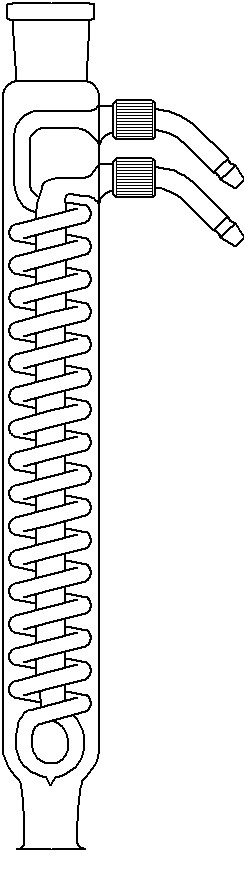
\includegraphics[height=5cm]{img/dimroth}
		\caption{\textsc{Dimroth}-Kühler}
		\label{fig:dimroth}
	\end{minipage}
\end{figure}
\FloatBarrier

\subsubsection*{Liebigkühler}
Der \textsc{Liebig}-Kühler ist ein Kühler bestehend aus einem Glasrohr mit Wassermantel. Er wird hauptsächlich als Kühler für Destillationsprodukte genutzt und kann auch unter Hochvakuum eingesetzt werden. Aufgrund der simplen Bauweise ist dieser Kühler zwar preiswert, leicht zu reinigen und robust, weist jedoch auch nur eine kleine Kühlfläche auf.
\begin{figure}[h!]
	\centering
	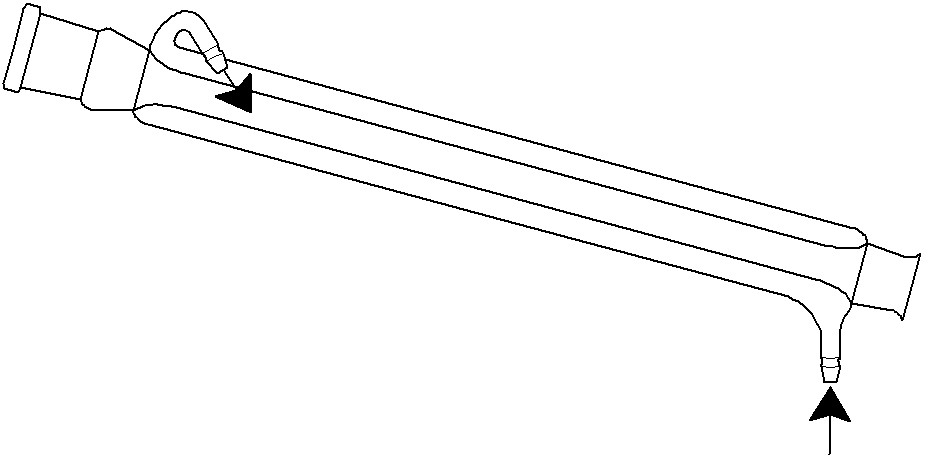
\includegraphics[width=0.4\textwidth]{img/liebigkuehler}
	\caption{\textsc{Liebig}-Kühler}
	\label{fig:liebigkuehler}
\end{figure}
\FloatBarrier

\subsection{Heiz- und Kühlelemente}
Um Proben oder Lösungen in Rundkolben, Reagenzgläsern oder Bechergläsern zu erwärmen oder abzukühlen eigenen sich verschiedene Mittel zur Umsetzung.



\subsubsection*{Heizbad und Eisbad}
Gerade wenn es darum geht Stoffe bzw. Proben schonend zu erwärmen, ist es ratsam ein Wasser oder Ölbad zu nutzen. Oft wird das Heizbad vorgewärmt und dann auf einer Heizplatte mit Magnetrührer warmgehalten. Ein typisches Öl für ein solches Heizbad ist Silikonöl.\\

\tipp{Tipp}{Wenn man nicht solange warten möchte bis das Wasser über eine Heizplatte anfängt zu sieden, sollte man einen handelsüblichen Wasserkocher nutzen. Diese finden sich mehrfach im Labor.}\\

\vspace*{7mm}

Ebenso wie das Aufheizen von Proben ist im chemischen Labor auf das Abkühlen von Proben notwendig. Hierfür wird in den meisten Fällen Eis oder auch einfach nur Leistungswasser genutzt.\\

\tipp{Tipp}{Möchte man, dass gerade ein Eisbad effizienter kühlte sollte dem Eisbad ein paar Millilieter Wasser zugegeben werden, um die Kontaktfläche zum jeweiligen Volumengefäß zu vergrößern. Sind zusätzlich Temperaturen des Eises von \SI{0}{\celsius} nötig, dann sollte dem Eis etwas Natriumchlorid zugegeben werden, um eine \textit{Kältemischung} herzustellen.}\\

\newpage

\subsubsection*{Heizpilz oder Heiznetz}
Heizpilze sind halbkugelförmige Heizmäntel mit eingehäkelten Heizleitern. Der Name Heiz\textsc{pilz} leitet sich dabei von der Marke \textsc{Pilz} ab.\\
Sie werden im Regelfall zur Erwärmung des Inhaltes von Rundkolben genutzt und besitzen meist eine Stufenweise Einstellmöglichkeit der Heizleistung. Heizpilze sind für Rundkolbenvolumina von \SI{50}{\milli \liter} bis \SI{20}{\liter} verfügbar.\\

\tipp{Wichtig}{Man sollte tunlichst vermeiden Flüssigkeiten oder Proben auf dem Heizpilz zu verschütten, um Kurzschlüsse oder Brände zu vermeiden !}\\

\subsubsection*{Heizplatte}
Heizplatte sind im chemischen Labor in Kombination mit Magnetrührern vorzufinden. Sie dienen zum direkten Erwärmen von Lösungen, Proben und Heizbad-Medien. \\
Gerade wenn leicht entzündliche Lösungen erhitzt werden sollen, ist jedoch von der Nutzung einer Heizplatte abzuraten ! Es sollten lieber alternative Heizelemente wie ein Heizpilz oder noch besser ein Heizbad genutzt werden.

\subsubsection*{Brenner}
Der typische Laborgasbrenner auch \textsc{Bunsen}-Brenner genannt, ist ein nach dem \textsc{Venturi}-Prinzip selbst-Luft-ansaugender Gasbrenner, welcher im chemischen Labor zum Erhitzen von Proben oder Flüssigkeiten genutzt wird.  Er sollte vorrangig dann genutzt werden, wenn keine leicht entzündlichen oder thermisch empfindlichen Stoffe genutzt werden und eine hohe Wärmebereitstellung erforderlich ist. Er in Kombination mit einem Dreifuß genutzt. Für qualitative Analysen, wie zum Beispiel der Flammfärbung oder oder Boraxperle findet er ebenfalls noch Verwendung.\\
In Abbildung \ref{fig:brenner} ist nochmals aufgeführt, welche Flammen am Brenner je nach Gaszufuhr und vorliegen welche Temperaturzonen in der rauschenden Flamme vorhanden sind.\\

\begin{figure}[h!]
	\centering
	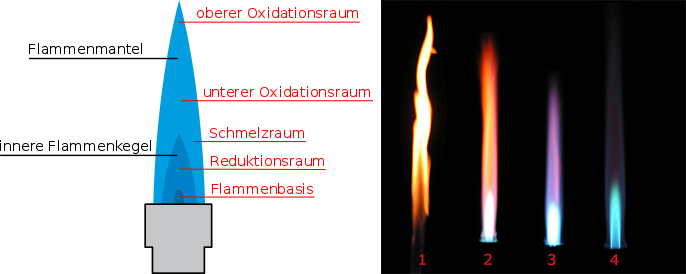
\includegraphics[width=0.75\textwidth]{img/brennerflamme3}
	\caption{Übersicht \textsc{Bunsen}-Brenner}
	\label{fig:brenner}
\end{figure}
\FloatBarrier

\subsection{Apparaturen zum Trocknen und Brennen}
\subsubsection*{Exsikkator}
Der Exsikkator ist ein Laborgerät, welches zur Trocknung chemischer Feststoffe verwendet wird. Der Behälter besteht meist aus einem dickwandigen Glas und kann mit einem Deckel luftdicht verschlossen werden. Falls notwendig kann dafür zusätzlich Schlifffett genutzt werden.\\
Exsikkatoren unterteilen sich zumeist in zwei Teile. In einen unteren Teil kleineren Durchmessers, um das jeweilige Trockenmittel wie zum Beispiel Calciumchlorid oder häufiger noch gefärbtes Silicagel (auch Kieselgel genannt) hineinzugeben und einen durch eine Siebplatte getrennten oberen Teil größeren Durchmessers in dem die Probe innerhalb eines Becherglases, einer Kristallisierschale oder einer Uhrglasschale hinein gestellt wird.\\
Prinzipiell entzieht im Exsikkator das Trockenmittel dem zu trocknenden Gut die Feuchtigkeit. Mittels Feuchtigkeitsindikator kann dann auf festgestellt werden wie stark das genutzte Trockenmittel bereits mit Wasser beladen ist.\\ 
Um Proben schneller zu trocknen, gibt es zum Teil auch Exsikkatoren, welche über einen Absperrhahn mit einer Vakuumpumpe verbunden werden können. Solche Exsikkatoren werden als \textit{Vakuumexsikkatoren} bezeichnet. Durch das Vakuum wird die Siedetemperatur des Wassers herabgesetzt und verdampft somit schneller.

\bild{Exsikkator}{.8}

\subsubsection*{Trockenschrank}
\begin{figure}[h!]
	\begin{minipage}[t]{0.65\textwidth}
		\vspace{0pt}
		Mit Trockenschränken können gleichzeitig mehrere Proben unter konstanten Temperatur und Feuchtigkeitsbedingungen getrocknet werden. Meistens wird dabei die Luft im Trockenschrank selbst entfeuchtet. Temperaturen sind in der Regel von der Raumtemperatur ausgehend bis \SI{250}{\celsius} möglich. Ausgehend von der Funktionsweise sind die meisten Trockenschränke ähnlich einem herkömmlichen Elektro-Backofen aufgebaut. 
	\end{minipage}
	\hfill
	\hspace{1mm}
	\begin{minipage}[t]{0.3\textwidth}
		\minibild{Trockenschrank}{0.9}{0pt}
	\end{minipage}
\end{figure}
\FloatBarrier

\subsubsection*{Muffelofen}
\begin{figure}[h!]
	\begin{minipage}[t]{0.65\textwidth}
		\vspace{0pt}
		Der Muffelofen ist ein Ofen in dem die Kammer mit dem zu brennenden/schmelzenden Gut durch einen hitzefesten Einsatz (die Muffel) getrennt ist. Als Einsatz werden meist feuerfeste Steine, wie Schamott (45 \% \ce{Al2O3}), eingesetzt.\\
		Im Labor werden Sie für verschiedene gravimetrische Verfahren in der Analytik genutzt oder in der Umwelttechnik und den Inertstoff- und den Kohlenstoffgehalt von Böden zu bestimmen. Aber auch für weitere Anwendungen des Schmelzens, Glühens und Veraschens können diese Öfen genutzt werden.
	\end{minipage}
	\hfill
	\hspace{1mm}
	\begin{minipage}[t]{0.3\textwidth}
		\minibild{Muffelofen}{0.9}{0pt}
	\end{minipage}
\end{figure}
\FloatBarrier

\subsection{Pumpen}
- Werden für Vakuum und Druck benutzt (Wann was sinnvoll)

Umwälzpumpe

\subsubsection*{Wasserstrahlpumpe}
- sind veraltet wegen Geräuschpegel und Wasserverbauch
- Druckbereich ?

\subsubsection*{Membranpumpe}
\subsubsection*{Drehschieberpumpe}
= Gleich Ölpumpe

\subsubsection{Schlauchpumpe}
Peristaltische Pumpe - Dosierpumpe

Verfahrenstechnik
\subsubsection*{Hubkolbenpumpe}
\subsubsection*{Kreiselpumpe}



\subsection{Füllkörper}

\subsection{Zusätzlich:}
\subsubsection*{Pyknometer}
\subsubsection*{Beschriftung von Proben}

%\subsubsection{\hypertarget{Normschliff}{Schliffe} und Schlifffett}
\subsubsection*{Schliffe und Schlifffett}
\label{sec:normschliff}
\subsubsection*{Ultraschallbad}
\subsubsection*{Eismaschine}
